\documentclass{article}

% Recommended, but optional, packages for figures and better typesetting:
\usepackage{microtype}
\usepackage{graphicx}
\usepackage{subfigure}
\usepackage{booktabs}
\usepackage{amsmath}

\usepackage{hyperref}

\newcommand{\theHalgorithm}{\arabic{algorithm}}

\usepackage[accepted]{icml2021}

\icmltitlerunning{A Masked DQN Agent for Two-Player Briscola}

\begin{document}

\twocolumn[
\icmltitle{A Masked DQN Agent for Two-Player Briscola}

\icmlsetsymbol{equal}{*}

\begin{icmlauthorlist}
\icmlauthor{Hermann Serain}{}
\end{icmlauthorlist}

\icmlkeywords{Reinforcement Learning, UniPD, Briscola, DQN}

\vskip 0.3in
]

\printAffiliationsAndNotice{}

\begin{abstract}
I train an agent for two-player Briscola with the goal of maximizing the win rate against the provided rule-based \texttt{ScriptedAIAgent}.
I first design a non-learning heuristic baseline built on card counting and expected-value reasoning, which wins $59.9\%$ of the games against the scripted opponent.
I then train a Deep Q-Network with action masking on the legal moves, filling the gaps in the provided codebase.
The learned agent reliably beats the scripted opponent ($52.3\%$ win rate over $1000$ evaluation games) but does not surpass my baseline.
As a bonus, I train the full $2 \times 2$ matrix \{DQN, A2C\} $\times$ \{standard, ``own points''\} reward: the algorithm choice dominates, with both A2C runs remaining near the luck floor while DQN is robust to the reward variant.
I analyze why, and discuss the improvements I consider most promising.
\end{abstract}

\section{Task and critical issues}
\label{sec:task}

Briscola is a two-player trick-taking card game played with a 40-card deck: at each turn both players play one card, the trick winner collects the card points ($120$ in total) and a game is won by exceeding $60$ points. The environment is provided; the agent observes a $244$-dimensional binary-ish state (turn features, its hand, the cards on the table and all cards seen so far, each with a briscola-suit flag) and outputs one of $40$ actions (card identities), of which only the cards actually in hand are legal. I identified the following critical issues.

\textbf{Imperfect information and stochasticity.} The opponent's hand and the deck order are hidden, so identical observed states can lead to different outcomes: the return of any fixed policy has high variance. This luck component has a measurable size: a uniformly random player still wins $21.2\%$ of games against the scripted agent (seed 0, $1000$ games). Win-rate estimates must therefore be read with a binomial error bar of about $\pm 1.5\%$ at $1000$ games, and learning curves are intrinsically noisy.

\textbf{Reward design.} The environment rewards the points of each trick ($\pm$ for winner/loser) rather than the game outcome. This is a dense and informative signal, but it is a proxy: maximizing expected points is not exactly maximizing win probability (e.g.\ winning $61$--$120$ points counts the same). I kept the provided reward (with \texttt{win\_extra\_points}$=0$) precisely because it is dense; the mismatch is discussed in Section~\ref{sec:discussion}.

\textbf{Legal-action masking.} The network scores all $40$ cards, but only the $1$--$3$ cards in hand are playable. Without restricting both the acted policy and the bootstrap target to legal moves, Q-learning propagates values of impossible actions and does not converge. Masking is applied in action selection and inside the TD target (Section~\ref{sec:algorithm}).

\textbf{Provided-code pitfalls.} The codebase is part of a larger project, and some provided components interact in subtle ways. The most consequential one: the training loop collects games with a \emph{greedy} clone of the agent (\texttt{clone()} defaults to \texttt{training=False}), silently disabling $\varepsilon$-greedy exploration. I fixed this with a subclass that clones the agent in training mode; without the fix the replay buffer only ever contains greedy self-confirming trajectories.

\section{Heuristic baseline}
\label{sec:baseline}

The baseline (\texttt{HeuristicAgent}, same interface as the scripted agent, no learning) improves on \texttt{ScriptedAIAgent} with two ingredients the latter lacks: \emph{card counting} and \emph{expected-value decisions}. It maintains a set of all card identities seen on the table since the game started (reset at each new game). At any moment it can therefore enumerate the \emph{unseen} cards: deck cards minus seen cards, minus its own hand, minus the revealed briscola card. Its decision rules, in priority order:

\textbf{When playing second} (cards on the table):
\begin{enumerate}
    \item \emph{Close the game if possible}: among the hand cards that win the trick, if capturing brings the total above $60$ points, play the cheapest sufficient one (non-briscola first, then lowest strength).
    \item \emph{Free capture}: if the trick can be won without spending a briscola, do it with the most valuable winning card (banking the most points at no cost).
    \item \emph{Paid capture}: if winning requires a briscola, spend the \emph{weakest} sufficient one, and only if the points on the table reach a threshold that scales with the value of the briscola spent: $3$ points for a pointless briscola (2, 4--7), $6$ for fante/cavallo/re ($2$--$4$ points), $10$ for asso or tre ($10$--$11$ points). This is an expected-value trade: a high briscola is a near-certain future trick, and should not be traded for less than its worth.
    \item Otherwise \emph{discard safely}: play the card that gives away the least (fewest points, then non-briscola, then lowest strength).
\end{enumerate}

\textbf{When playing first}: lead the most valuable \emph{safe} card, where a lead is safe if \emph{no unseen card can beat it} --- a worst-case check against every card the opponent might hold. Safe leads with at least $3$ points bank guaranteed points; if no such lead exists, fall back to the safest discard, which preserves briscole and carichi.

The baseline is deterministic given the game state and runs in negligible time. Over $1000$ games (seed 0) it wins $\mathbf{59.9\%}$ against \texttt{ScriptedAIAgent} and $83.9\%$ against the random player. It is intentionally strong: card counting with worst-case safety reasoning is close to how good human players actually play, and it sets an informative (if demanding) bar for the learned agent.

\section{RL algorithm}
\label{sec:algorithm}

I chose \textbf{DQN} \cite{mnih2015dqn} among the two options supported by the codebase (DQN or A2C), for three reasons. First, the action space is small and discrete ($40$ actions, $\leq 3$ legal), the natural regime of value-based methods, and the legal-action mask integrates exactly in both action selection and the bootstrap target --- whereas masking a softmax policy requires more care. Second, the opponent is \emph{fixed}, so the environment is stationary and the convergence setting of Q-learning applies; there is no need for the on-policy machinery of A2C. Third, experience replay reuses each simulated game many times, which matters on a CPU-only budget where game simulation is the bottleneck. Section~\ref{sec:bonus} tests this choice empirically.

The Q-network is a plain MLP $244 \to 256 \to 256 \to 40$ (ReLU, linear output head). Given transitions $(s, a, r, s', d)$ with legal-action masks $m'$ for $s'$, the loss on a minibatch is
\begin{equation}
    \mathcal{L}(\theta) = \Big( r + \gamma \, (1-d) \max_{a' :\, m'(a')=1} Q_{\theta^-}(s', a') - Q_\theta(s, a) \Big)^{\!2}
\end{equation}
where $\theta^-$ is a frozen target network. The masked $\max$ is implemented by adding $-\infty$ (float min) to the Q-values of illegal actions before the maximum: the target only ever bootstraps from moves that are actually available, which I found indispensable for convergence.

\textbf{Training setup} (seed 0 for \texttt{random}, NumPy and TensorFlow): $6000$ epochs of $1$ game each against \texttt{ScriptedAIAgent}; replay buffer of $10^4$ transitions; $2$ gradient updates per epoch with batch size $128$; Adam with learning rate $10^{-3}$; MSE loss; target network refreshed every $250$ training iterations; $\gamma = 1$ (episodes are short and finite, so no discount is needed); $\varepsilon$-greedy exploration decaying linearly from $1.0$ to $0.1$ at $80\%$ of training and constant afterwards. Every $250$ epochs the greedy policy is evaluated over $500$ games against the scripted and random opponents, and the weights are checkpointed.

\section{Results}
\label{sec:results}

Figure~\ref{fig:learning-curve} shows the learning curve. The agent surpasses the random-play level almost immediately, crosses the $50\%$ mark against the scripted opponent around epoch $2000$, and then plateaus in the $0.51$--$0.55$ band, with the best checkpoint at epoch $5250$ ($0.556$ over the $500$-game running evaluation). The dashed horizontal lines are the baseline of Section~\ref{sec:baseline}, which the curve does not reach.

\begin{figure}[ht]
\vskip 0.2in
\begin{center}
\centerline{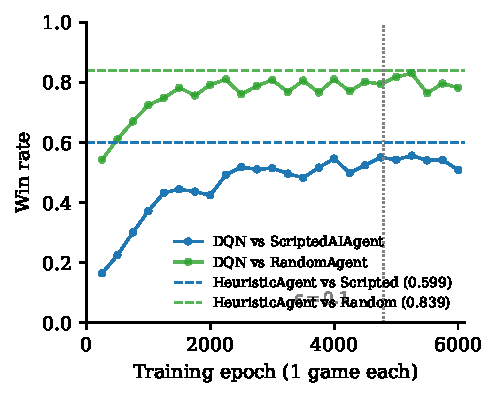
\includegraphics[width=\columnwidth]{learning_curve}}
\caption{Win rate of the greedy DQN policy during training, evaluated every $250$ epochs over $500$ games against the scripted (blue) and random (green) opponents. Dashed lines: the heuristic baseline against the same opponents. Dotted vertical line: end of the $\varepsilon$ decay.}
\label{fig:learning-curve}
\end{center}
\vskip -0.2in
\end{figure}

For the final evaluation I selected the best checkpoint and re-evaluated it greedily over $1000$ fresh games per opponent (seed 0, \texttt{python evaluate.py}); Table~\ref{tab:results} summarizes all agents under the same protocol. The learned agent wins $\mathbf{52.3\%}$ of games against the scripted opponent (average $61.6$ points per game vs.\ $58.3$) and $79.1\%$ against the random player. The gap between the $500$-game running evaluation ($55.6\%$) and the $1000$-game final one ($52.3\%$) is consistent with the $\pm 2\%$ binomial noise of the two estimates.

\begin{table}[t]
\caption{Win rates over $1000$ games, seed 0. Rows: evaluated agent; columns: opponent.}
\label{tab:results}
\vskip 0.15in
\begin{center}
\begin{small}
\begin{sc}
\begin{tabular}{lcc}
\toprule
Agent & vs Scripted & vs Random \\
\midrule
RandomAgent     & 21.2\% & --     \\
ScriptedAIAgent & --     & 78.8\% \\
DQN (this work)      & 52.3\% & 79.1\% \\
HeuristicAgent (this work) & \textbf{59.9\%} & \textbf{83.9\%} \\
\bottomrule
\end{tabular}
\end{sc}
\end{small}
\end{center}
\vskip -0.1in
\end{table}

\section{Bonus experiments: A2C and reward design}
\label{sec:bonus}

To separate the contribution of the algorithm from that of the reward, I trained the full $2 \times 2$ matrix \{DQN, A2C\} $\times$ \{standard, own-points reward\} under the same protocol of Section~\ref{sec:algorithm} (seed 0, $6000$ epochs, running evaluation every $250$ epochs).

\textbf{A2C.} Actor and critic share the DQN body ($284 \to 256 \to 256$; softmax over the $40$ actions, resp.\ scalar value). The policy is masked and renormalized over the legal cards, both when acting and inside the loss $-\mathbb{E}[A \log \pi(a|s)]$, with an entropy bonus ($\beta = 0.01$); the advantage $A = G - V(s)$ uses Monte-Carlo returns $G$ (episodes are short, and the exact return does not depend on a critic still learning), is treated as a constant and normalized per batch; evaluation plays the mode of the policy. Being on-policy, A2C has no replay buffer: each batch of transitions is consumed right after being collected ($4$ passes), so at equal simulation budget it performs roughly $40\times$ fewer gradient steps than DQN.

\textbf{Own-points reward.} The variant rewards the trick winner with the trick points and gives the loser $0$: with $\gamma = 1$ the return is exactly the agent's final score ($0$--$120$) instead of the point differential ($\pm 120$), removing the explicit incentive to deny points to the opponent.

\begin{figure}[ht]
\vskip 0.2in
\begin{center}
\centerline{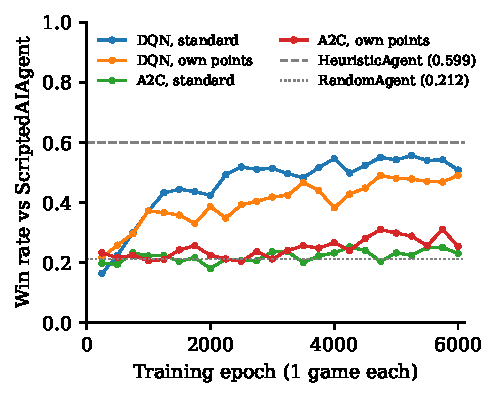
\includegraphics[width=\columnwidth]{learning_curve_bonus}}
\caption{Win rate against \texttt{ScriptedAIAgent} during training for the four configurations (running evaluation, $500$ games every $250$ epochs). Dashed: heuristic baseline; dotted: random-play luck floor.}
\label{fig:bonus-curve}
\end{center}
\vskip -0.2in
\end{figure}

% Numbers = running evaluations (500 games) stored in win_rates.txt.
% Optionally add a 1000-game column from: python evaluate.py --agent {dqn,a2c} --reward {standard,own}
\begin{table}[t]
\caption{Bonus matrix: win rate vs \texttt{ScriptedAIAgent} on the $500$-game running evaluation (best checkpoint, with its epoch, and final).}
\label{tab:bonus}
\vskip 0.15in
\begin{center}
\begin{small}
\begin{sc}
\begin{tabular}{lcc}
\toprule
Configuration & Best (epoch) & Final \\
\midrule
DQN, standard   & \textbf{0.556} (5250) & 0.508 \\
DQN, own points & 0.490 (6000) & 0.490 \\
A2C, standard   & 0.252 (4250) & 0.230 \\
A2C, own points & 0.310 (5750) & 0.254 \\
\bottomrule
\end{tabular}
\end{sc}
\end{small}
\end{center}
\vskip -0.1in
\end{table}

Figure~\ref{fig:bonus-curve} and Table~\ref{tab:bonus} give three clear answers. \emph{(i) The algorithm dominates the reward}: both DQN runs climb into the $0.45$--$0.55$ band, both A2C runs remain within $\sim\!0.1$ of the $21\%$ luck floor. \emph{(ii) A2C fails for the reasons anticipated in Section~\ref{sec:algorithm}}: far fewer gradient steps per simulated game, and a policy-gradient signal whose variance is inflated by the luck component. The failure mode is policy collapse: in the own-points run the softmax saturated around epoch $1000$ (probability $\approx 1$ on a single action, legal-card probabilities underflowing to $0$), to the point of requiring a numerical guard in action selection. \emph{(iii) Reward design is second-order}: the own-points variant slightly hurts DQN ($0.490$ vs.\ $0.556$ at best), consistent with losing the defensive information carried by the negative rewards, and slightly helps the (much weaker) A2C, but neither effect approaches the algorithm gap.

\section{Discussion}
\label{sec:discussion}

\textbf{The task goal is met, the internal bar is not.} The DQN beats the opponent it was asked to beat: $52.3\%$ against \texttt{ScriptedAIAgent}, with a positive point differential, and it plays at the scripted agent's own level against the random player ($79.1\%$ vs.\ $78.8\%$). It does not, however, surpass my heuristic baseline. I believe the main reason is that the baseline was built deliberately strong: it receives, for free and in exact symbolic form, precisely the two quantities that are hardest to extract from the flat $244$-dimensional observation --- the set of still-unseen cards and a worst-case comparison of every hand card against that set. The network sees the same information in principle (the state includes all cards seen so far), but must rediscover counting and worst-case reasoning implicitly in its weights from a noisy, high-variance reward signal.

\textbf{Why the plateau.} Three compounding causes are plausible. (i) \emph{Return variance}: with a $\sim 21\%$ luck floor, the Bellman targets of near-tied states are dominated by noise that more games per update would average out. (ii) \emph{Proxy reward}: the agent maximizes expected points, and the plateau band is exactly where converting extra points into extra \emph{wins} requires endgame-specific play (e.g.\ point $61$ is worth everything, point $100$ nothing extra) --- although the own-points experiment of Section~\ref{sec:bonus} shows that re-designing the dense reward alone does not move the plateau. (iii) \emph{Max-operator overestimation}, amplified by $\gamma=1$ and MSE on rewards in the $\pm 21$ range.

\nocite{sutton2018reinforcement}

\bibliography{main}
\bibliographystyle{icml2021}

\end{document}
